 \documentclass{article}

\usepackage[francais]{babel}
\def\printlandscape{\special{landscape}}    % Works with dvips.
%\usepackage{pstricks,pst-node,pst-tree}
%\usepackage{amssymb}
\usepackage{amsmath}
\usepackage[utf8]{inputenc}
\usepackage[T1]{fontenc} 
\usepackage{fancybox} % for shadow and Bitemize
\usepackage{alltt}
\usepackage{graphicx}
%\usepackage{epsfig}
%\usepackage{fullpage}
%\usepackage{fancyhdr}
%\usepackage{moreverb}
%\usepackage{xspace}
\usepackage[colorlinks,hyperindex,bookmarks,linkcolor=blue,citecolor=blue,urlcolor=blue]{hyperref}

\usepackage{wrapfig}
\usepackage{epsf}
\usepackage{enumitem}
\usepackage{pifont}

\begin{document}

\title{Rapport de projet pluridisciplinaire}

\date{\today}
        
\newpage

\title{Diffusion non linéaire en sciences de la terre modélisation des glaciers}
 
\maketitle
\tableofcontents

\begin{abstract}
Résumé du contenu du document.
\end{abstract}

%-----------------------------------------------------------
\newpage
\section{Introduction}\label{sec:intro}

L’écoulement des glaciers est un processus continu, mais il est très difficile de le simuler mathématiquement. Pour cela, les modélisateurs utilisent des méthodes numériques, qui résolvent les équations en une série d’étapes.
L’intérêt ici va être d’énoncer les relations générales de Stokes appliqués aux glaciers, d’énoncer le modèle Shallow Ice Approximation (SIA) afin d’en déterminer les avantages et les limites dans l’analyse de l’écoulement d’un glacier en fonction du temps.

L’écoulement d’un glacier dépend de plusieurs facteurs, qui sont principalement l’accumulation de neige, la fonte de glace, la gravité et le niveau de la pente du lit rocheux.
Les écoulements sont considérés comme fluides, incompressibles, visqueux et non linéaires, d’où l’intérêt de les modéliser avec les relations de Stokes.
Dans le cadre de ce projet, nous allons utilisé le langage Julia pour la résolution de systèmes d'équations différentielles afin de pouvoir prédire l'écoulement glaciaire du Groenland.


%-----------------------------------------------------------
\section{Présentation des techniques de résolution}

\subsection{Pourquoi Julia ?}

Julia est un langage de programmation moderne et polyvalent, crée en 2009 par des chercheurs et ouvert au grand public en 2012. C'est un langage de haut niveau, dynamique et conçu pour des calculs scientifique. Sa syntaxe est similaire à Python, R ou encore Matlab.
 


\subsection{Les équations de Stokes}

https://scienceetonnante.com/2014/03/03/la-mysterieuse-equation-de-navier-stokes/
https://hal.uca.fr/hal-03022007/document

Les équations de Stokes ont comme principal objectif de décrire les mouvements des fluides. 
Pour décrire correctement un fluide en mouvement, il faut connaître sa vitesse en tout point de l'espace : son champ de vitesse. Ainsi les équations de Stokes permettent de décrire le champ de vitesse d'un fluide. 
Dans un fluide nous considérons deux types de forces à savoir, les forces de pression et les forces visqueuses. 

Afin de pouvoir appliquer ces équations dans le cas des écoulements des glaciers, nous considérerons ces derniers comme des fluides incompressibles, visqueux et non linéaires. Il s'agit d'un système d'équations pouvant être appliqué à tout type de glacier.

Ce système permet une très grande précision dans les résultats puisqu'il prend en compte toutes les contraintes au nombre de neuf, qu’elles soient longitudinales, transversales, verticales ou encore horizontales. 
Résoudre les équations de stokes revient à résoudre ce système : 


\begin{center}
$\left\{
\begin{array}{l}
-div(2 \mu ||\epsilon(\vec{v})||) + \nabla p = \rho \vec{g} \qquad(1)  \\
div(\vec{v}) = 0 \qquad
\end{array}
\right.$
\end{center}

avec $\vec{v}$ la vitesse, $\nabla p$ le gradient de pression, $\vec{g}$ l'accélération de pesanteur et $\rho$ la masse volumique.

Néanmoins, le Groenland  une calotte tellement grande de milliers de kilomètres, qu'il faut un nombre considérable de points pour résoudre ces équations. De plus du fait de la complexités des equations et des géométries de la calotte, cela est coûteux en temps de calcul. 

Nous observons que les calottes sont relativement mince, soit quelques kilomètres d'épaisseur, ainsi nous pouvons négliger les variations verticales de la vitesse / les contraintes de cisaillement longitudinal. Nous en concluons, que pour minimiser le temps de calcul, nous ne sommes pas obligé d'utiliser un modèle en 3D en résolvant les équations de Stokes mais que nous pouvons simplement utilisé un modèle simplifié en 2D. Le modèle SIA intervient justement en tant qu’approximation des relations de Stokes, permettant des calculs beaucoup plus simples pour un modèle en 2D.

 
\subsection{Shallow ice approximation (SIA)}
https://tel.archives-ouvertes.fr/tel-00192512v2/document

Nous avons vu que la résolution du systèmes des équations de Stokes est très couteuse en temps pour des applications réalistes. C'est pour cette raison que nous allons utiliser une simplification de ces équations basée sur le fait que sur de très grandes calottes, l'épaisseur est extrêmement faible par rapport à la dimension horizontal. Pour cela, nous allons utilisé le modèle SIA (shallow ice approximation). Sa validité dépend du rapport d'aspect caractéristique $\zeta$ des objets glaciaires :
\begin{center}
$\zeta = \frac{e}{L} \qquad(2)$
\end{center}

avec e l'épaisseur du glacier et L la largeur du glacier. Ce rapport est par exemple de $10^{-3}$ pour l'Antarctique et de $5.10^{-3}$ pour le Groenland. En effet, la validité de la SIA diminue lorsque le rapport d'aspect caractéristique $\zeta$ augmente. 
La SIA est en réalité la résolution d'une équation de diffusion non linéaire : 


\begin{center}
$\frac{\partial H}{\partial t}=D\frac{{\partial}^{2}H}{\partial x^{2}} + M\qquad(3)$
\end{center}

avec D le coefficient de diffusion, H l'épaisseur du glacier et M la masse balance.
\\

\begin{itemize}[label=\ding{212}]
\item H la hauteur du glacier 

L'épaisseur H est donnée par l'équation suivante : 
\begin{center}
$H(x) = S(x) + B(x)\qquad(4)$
\end{center}
où B est la hauteur de l'encaissant rocheux et S la topographie de la glace. H est représentée sur la figure ci-dessous : 
\\
\\
\begin{figure}[!htpb]
\centering
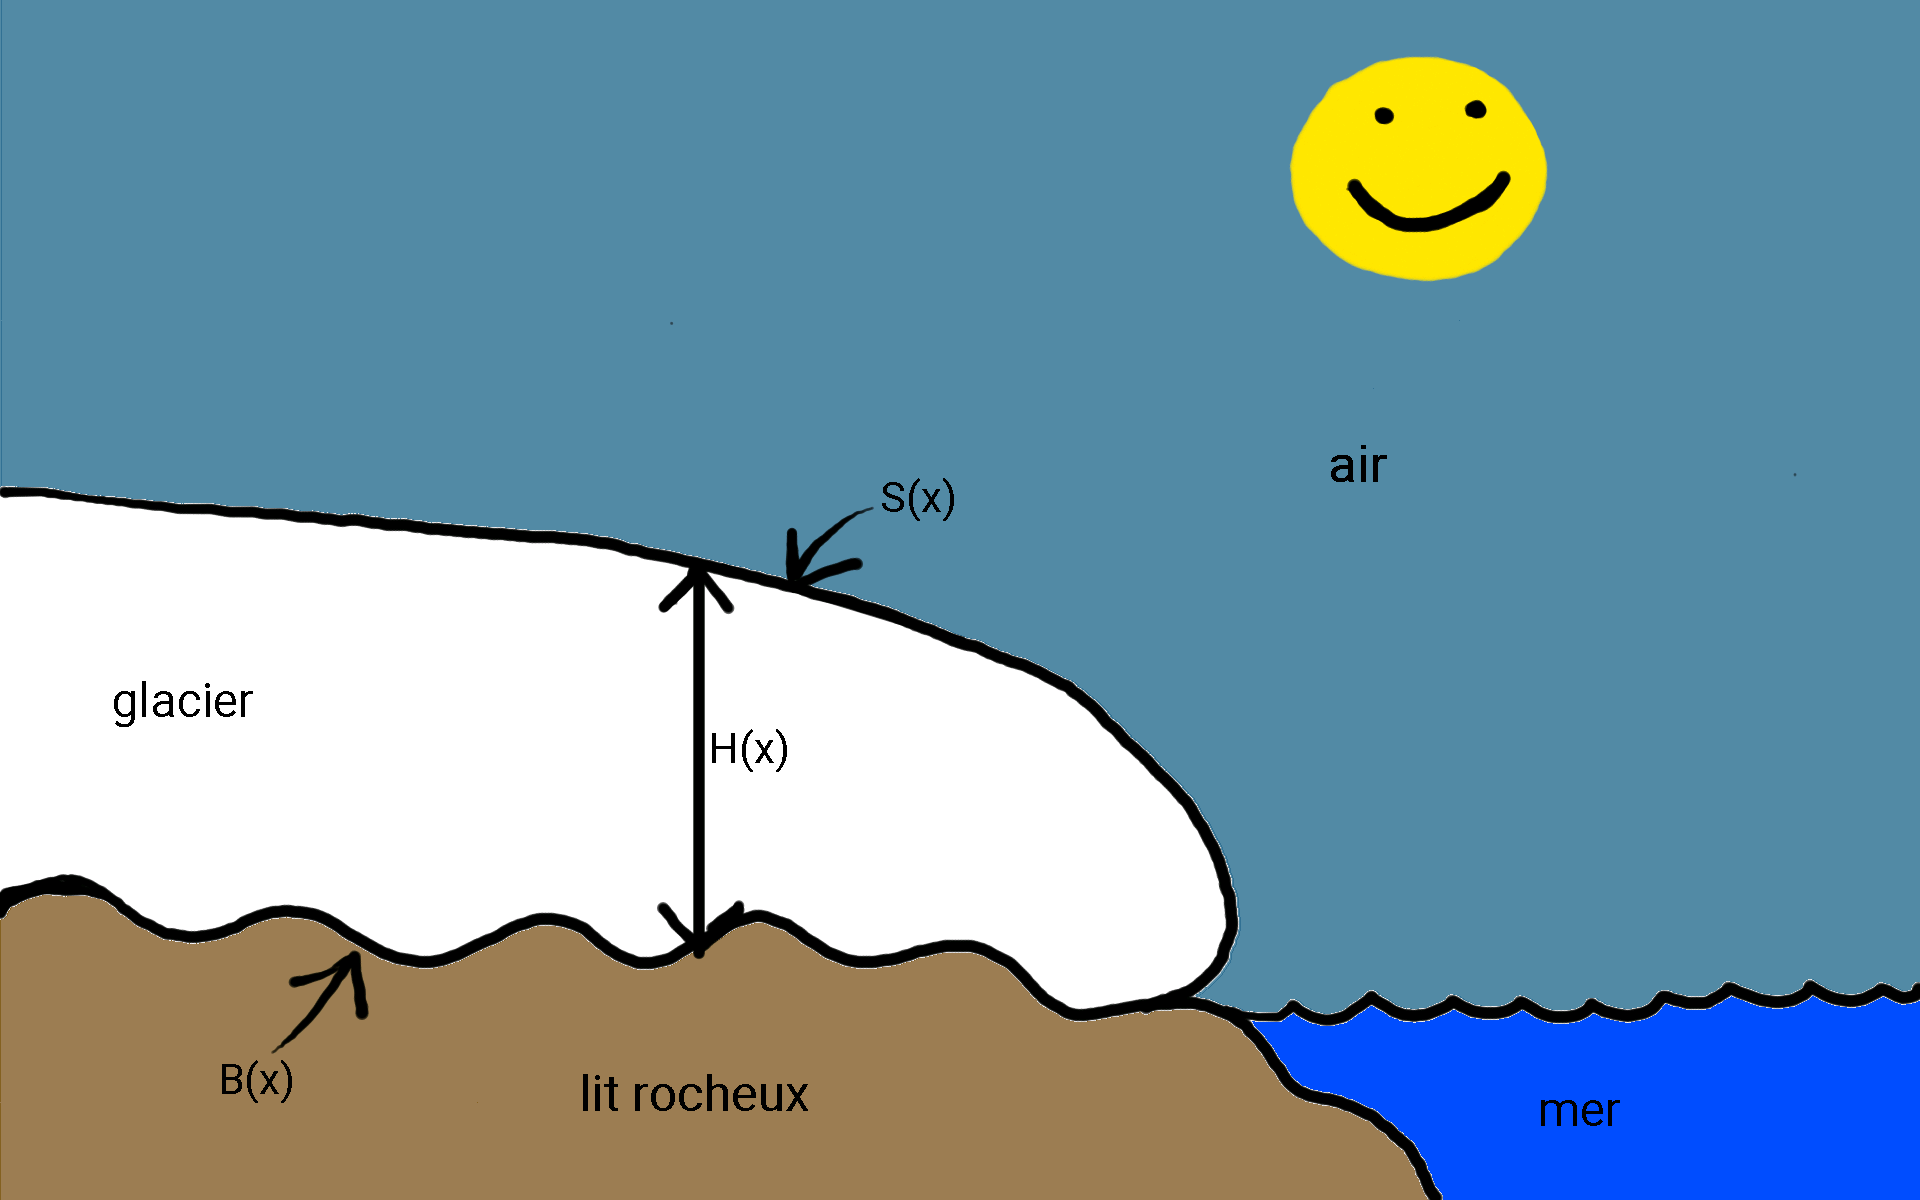
\includegraphics[width=10cm, keepaspectratio=true, height=10cm]{H.png}
\caption{Représentation de H, B et S}
\label{fig01ch1}
\end{figure}
\\

Les données topographiques, l'élévation du substratum rocheux et l'épaisseur de la glace proviennent du jeu de données BedMachine Greenland v3. 
\\
\item M la masse balance  

Il faut savoir que l'écoulement d'un glacier dépend de plusieurs facteurs : la neige, glace, pluie, fonte, perte de glace, gravité. La masse balance M est la somme de phénomène qui sont l'accumulation et l'ablation de la glace :
\begin{center}
$M = accumulaiton + ablation\qquad(5)$
\end{center}
Ainsi la masse balance permet d'équilibrer les 2 phénomènes à la surface en fonction de la ligne d'équilibre. L'altitude de la ligne d'équilibre (ELA) est où la zone d'accumulation, au sommet du glacier, est égale à la zone d'ablation, en bas du glacier. Nous pouvons la distinguer sur la figure ci-dessous : 
\begin{figure}
\centering
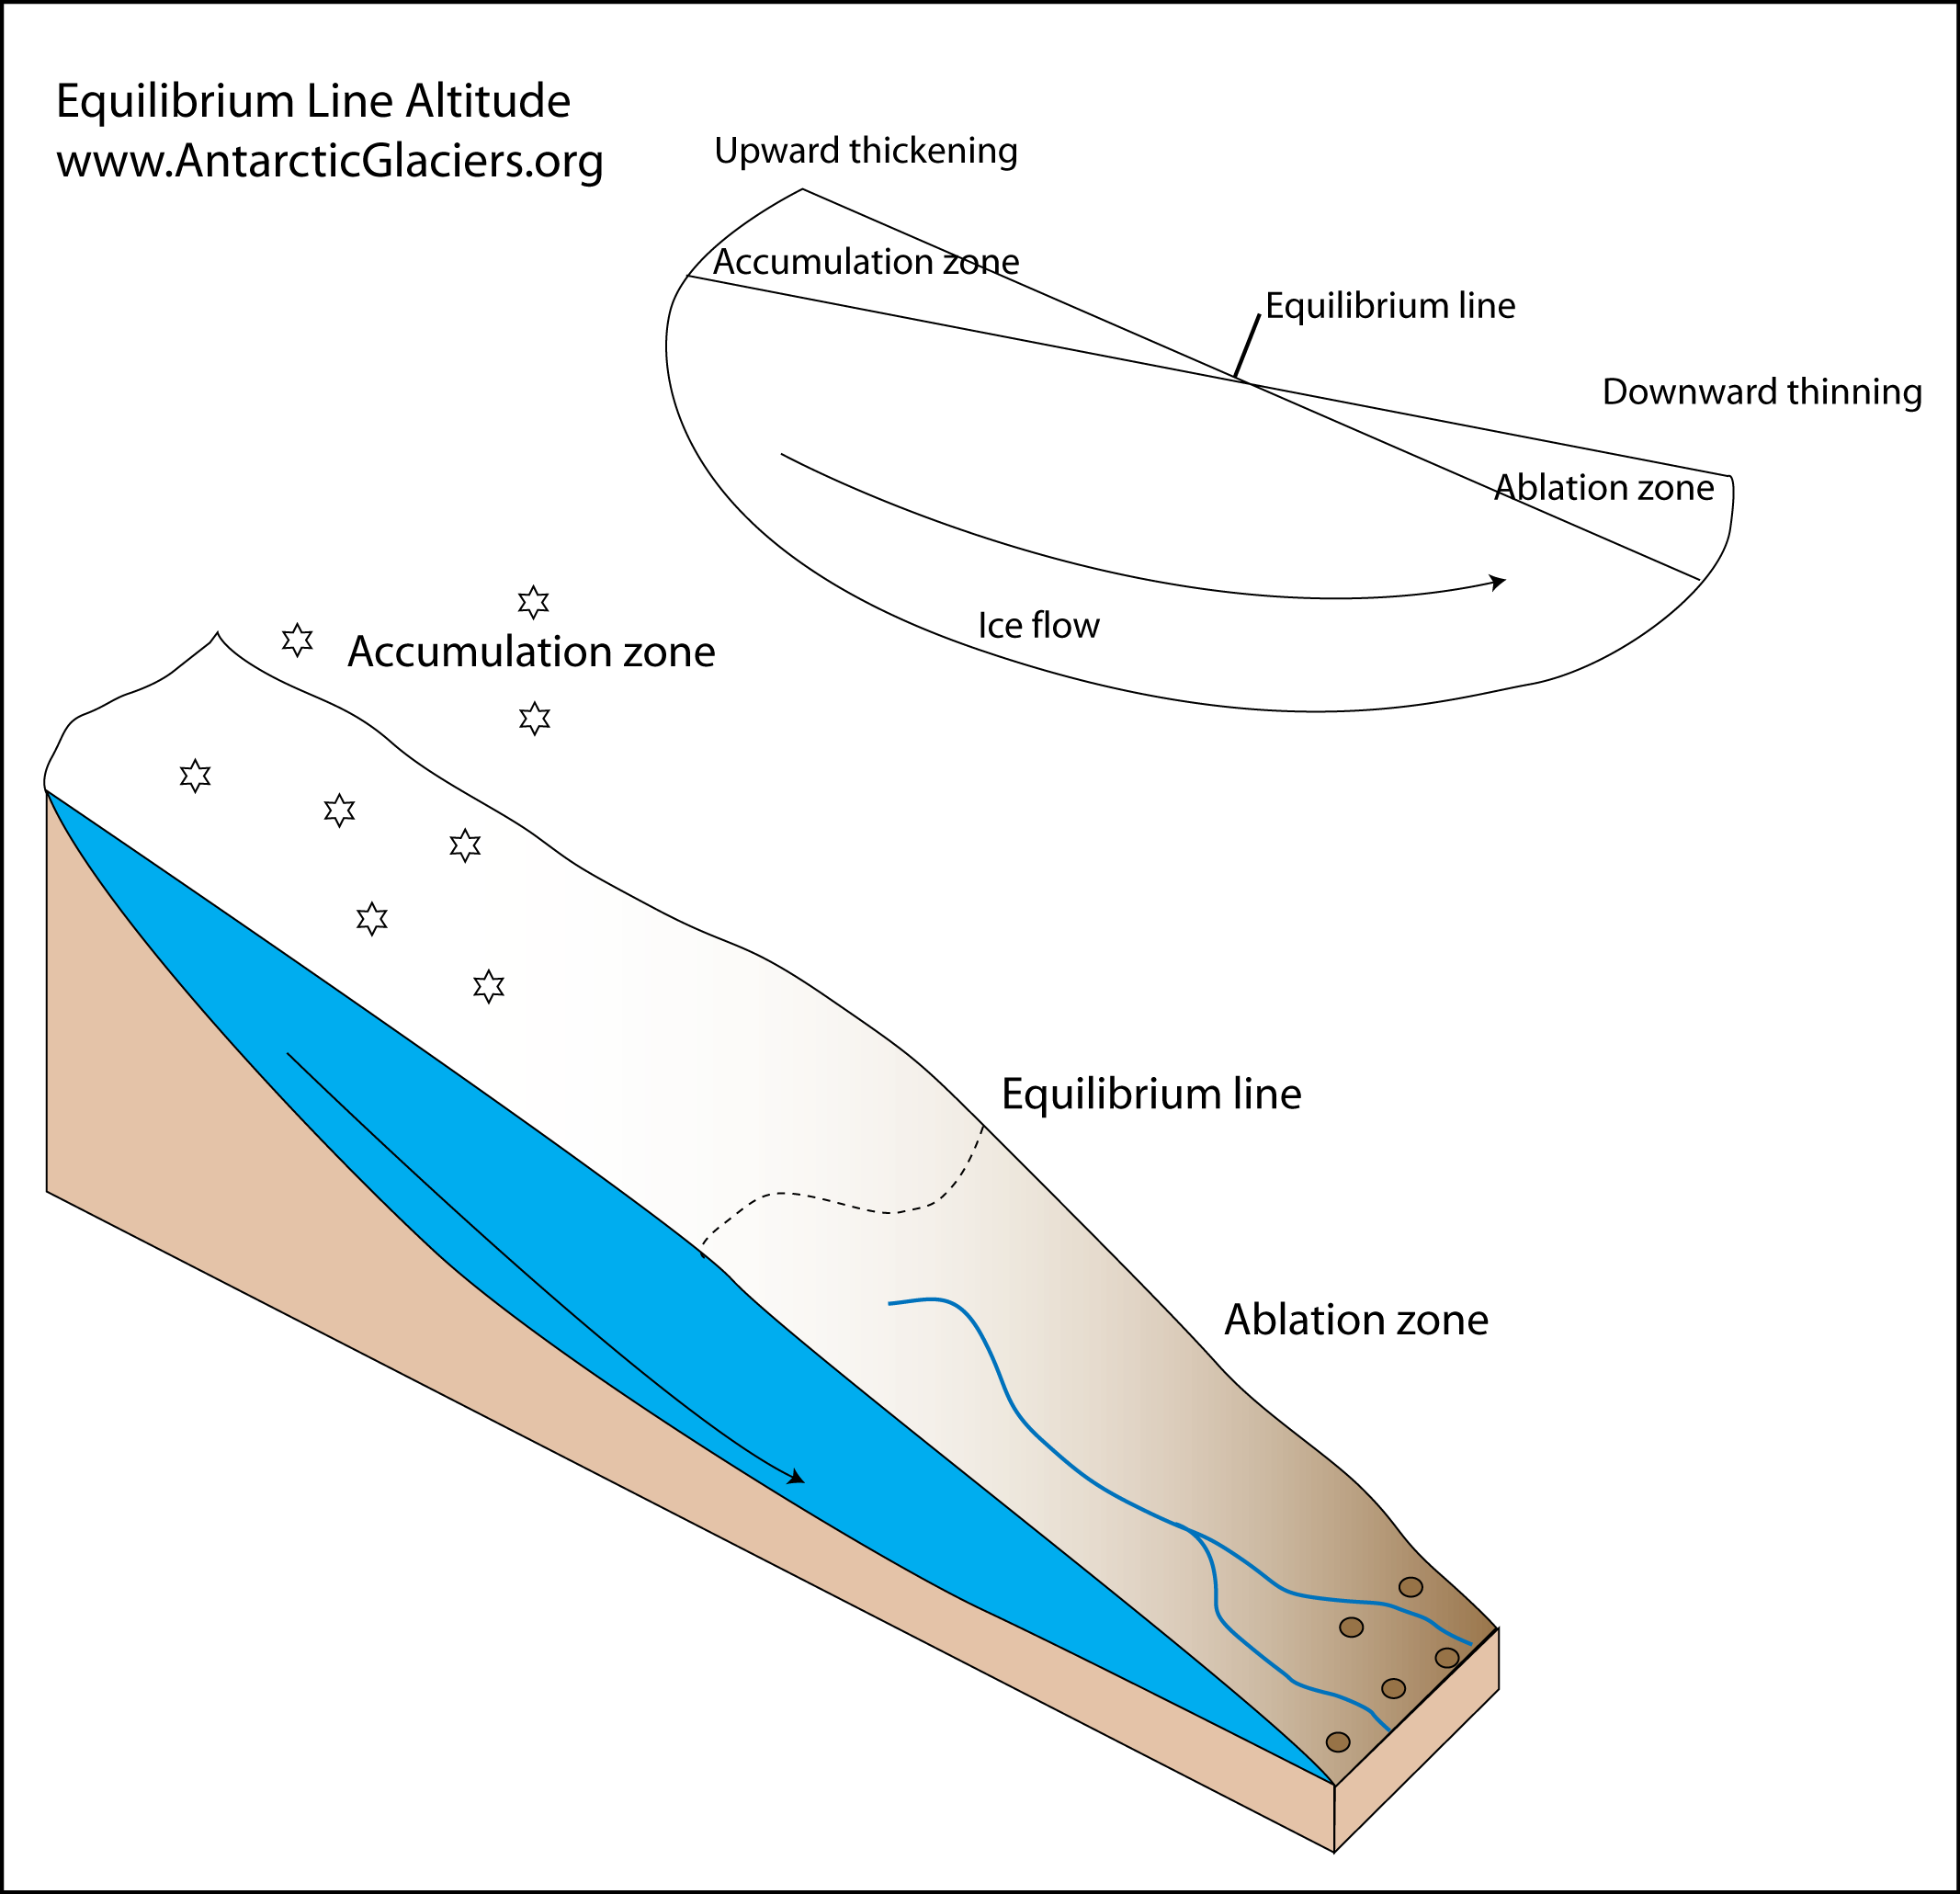
\includegraphics[width=10cm, keepaspectratio=true, height=9cm]{equilibrium_line_altitude1.png}
\caption{Représentation de la ligne d'équilibre sur un glacier}

\end{figure}

\end{itemize}

\newpage
Dans le code, la masse balance M est calculé à partir de gradb le gradient du bilan massique, zELA la latitude de la ligne d'équilibre (ELA) et bmax l'accumulation maximale.
\section{Simulations numériques}

\section{Résultats}

%-----------------------------------------------------------
\bibliography{rapport}
\bibliographystyle{abbrv}
\end{document}

%%% Local Variables:
%%% mode: latex
%%% TeX-master: t
%%% coding: utf-8
%%% End:
